\chapter{Recorrido de grafos}

Este capítulo discute dos algoritmos fundamentales
de grafos:
búsqueda en profundidad (DFS, por sus siglas en inglés) y búsqueda en anchura (BFS, por sus siglas en inglés).
Ambos algoritmos reciben un nodo de inicio
en el grafo,
y visitan todos los nodos que se pueden alcanzar
desde el nodo de inicio.
La diferencia en los algoritmos radica en el orden
en el que visitan los nodos.

\section{Búsqueda en profundidad}

\index{búsqueda en profundidad}

\key{Búsqueda en profundidad} (DFS)
es una técnica sencilla de recorrido de grafos.
El algoritmo comienza en un nodo inicial,
y procede a todos los demás nodos que son
alcanzables desde el nodo inicial utilizando
las aristas del grafo.

La búsqueda en profundidad siempre sigue un solo
camino en el grafo mientras encuentre
nodos nuevos.
Después de esto, regresa a los nodos anteriores
y comienza a explorar otras partes del grafo.
El algoritmo mantiene un registro de los nodos visitados,
de modo que procesa cada nodo solo una vez.

\subsubsection*{Ejemplo}

Consideremos cómo la búsqueda en profundidad procesa
el siguiente grafo:
\begin{center}
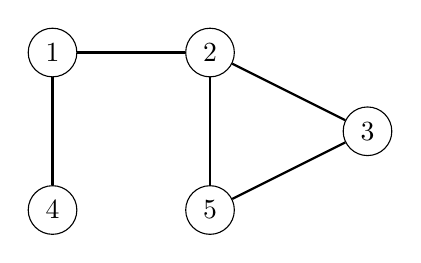
\begin{tikzpicture}
\node[draw, circle] (1) at (1,5) {$1$};
\node[draw, circle] (2) at (3,5) {$2$};
\node[draw, circle] (3) at (5,4) {$3$};
\node[draw, circle] (4) at (1,3) {$4$};
\node[draw, circle] (5) at (3,3) {$5$};

\path[draw,thick,-] (1) -- (2);
\path[draw,thick,-] (2) -- (3);
\path[draw,thick,-] (1) -- (4);
\path[draw,thick,-] (3) -- (5);
\path[draw,thick,-] (2) -- (5);
\end{tikzpicture}
\end{center}
Podemos comenzar la búsqueda en cualquier nodo del grafo;
ahora comenzaremos la búsqueda en el nodo 1.

La búsqueda primero avanza al nodo 2:
\begin{center}
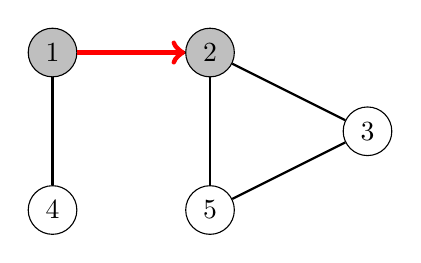
\begin{tikzpicture}
\node[draw, circle,fill=lightgray] (1) at (1,5) {$1$};
\node[draw, circle,fill=lightgray] (2) at (3,5) {$2$};
\node[draw, circle] (3) at (5,4) {$3$};
\node[draw, circle] (4) at (1,3) {$4$};
\node[draw, circle] (5) at (3,3) {$5$};

\path[draw,thick,-] (1) -- (2);
\path[draw,thick,-] (2) -- (3);
\path[draw,thick,-] (1) -- (4);
\path[draw,thick,-] (3) -- (5);
\path[draw,thick,-] (2) -- (5);

\path[draw=red,thick,->,line width=2pt] (1) -- (2);
\end{tikzpicture}
\end{center}
Después de esto, se visitarán los nodos 3 y 5:
\begin{center}
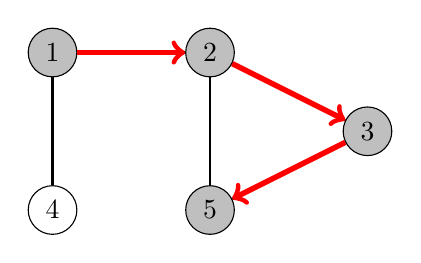
\begin{tikzpicture}
\node[draw, circle,fill=lightgray] (1) at (1,5) {$1$};
\node[draw, circle,fill=lightgray] (2) at (3,5) {$2$};
\node[draw, circle,fill=lightgray] (3) at (5,4) {$3$};
\node[draw, circle] (4) at (1,3) {$4$};
\node[draw, circle,fill=lightgray] (5) at (3,3) {$5$};

\path[draw,thick,-] (1) -- (2);
\path[draw,thick,-] (2) -- (3);
\path[draw,thick,-] (1) -- (4);
\path[draw,thick,-] (3) -- (5);
\path[draw,thick,-] (2) -- (5);

\path[draw=red,thick,->,line width=2pt] (1) -- (2);
\path[draw=red,thick,->,line width=2pt] (2) -- (3);
\path[draw=red,thick,->,line width=2pt] (3) -- (5);
\end{tikzpicture}
\end{center}
Los vecinos del nodo 5 son 2 y 3,
pero la búsqueda ya ha visitado ambos,
por lo que es hora de regresar a los nodos anteriores.
Además, los vecinos de los nodos 3 y 2
ya han sido visitados, por lo que luego nos movemos
del nodo 1 al nodo 4:
\begin{center}
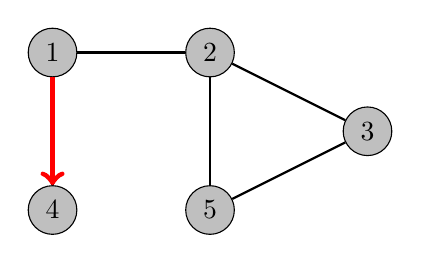
\begin{tikzpicture}
\node[draw, circle,fill=lightgray] (1) at (1,5) {$1$};
\node[draw, circle,fill=lightgray] (2) at (3,5) {$2$};
\node[draw, circle,fill=lightgray] (3) at (5,4) {$3$};
\node[draw, circle,fill=lightgray] (4) at (1,3) {$4$};
\node[draw, circle,fill=lightgray] (5) at (3,3) {$5$};

\path[draw,thick,-] (1) -- (2);
\path[draw,thick,-] (2) -- (3);
\path[draw,thick,-] (1) -- (4);
\path[draw,thick,-] (3) -- (5);
\path[draw,thick,-] (2) -- (5);

\path[draw=red,thick,->,line width=2pt] (1) -- (4);
\end{tikzpicture}
\end{center}
Después de esto, la búsqueda termina porque ha visitado
todos los nodos.

La complejidad temporal de la búsqueda en profundidad es $O(n+m)$
donde $n$ es el número de nodos y $m$ es el
número de aristas,
porque el algoritmo procesa cada nodo y arista una vez.

\subsubsection*{Implementación}

La búsqueda en profundidad se puede implementar de manera conveniente
utilizando recursión.
La siguiente función \texttt{dfs} comienza
una búsqueda en profundidad en un nodo dado.
La función asume que el grafo está
almacenado como listas de adyacencia en un arreglo
\begin{lstlisting}
vector<int> adj[N];
\end{lstlisting}
y también mantiene un arreglo
\begin{lstlisting}
bool visitado[N];
\end{lstlisting}
que mantiene un registro de los nodos visitados.
Inicialmente, cada valor en el arreglo es \texttt{false},
y cuando la búsqueda llega al nodo $s$,
el valor de \texttt{visitado}[$s$] se convierte en \texttt{true}.
La función se puede implementar de la siguiente manera:
\begin{lstlisting}
void dfs(int s) {
    if (visitado[s]) return;
    visitado[s] = true;
    // procesar el nodo s
    for (auto u: adj[s]) {
        dfs(u);
    }
}
\end{lstlisting}

\section{Búsqueda en anchura}

\index{búsqueda en anchura}

\key{Búsqueda en anchura} (BFS) visita los nodos
en orden creciente de su distancia
desde el nodo de inicio.
Por lo tanto, podemos calcular la distancia
desde el nodo de inicio a todos los demás
nodos utilizando búsqueda en anchura.
Sin embargo, la búsqueda en anchura es más difícil
de implementar que la búsqueda en profundidad.

La búsqueda en anchura recorre los nodos
un nivel tras otro.
Primero la búsqueda explora los nodos cuya
distancia desde el nodo de inicio es 1,
luego los nodos cuya distancia es 2, y así sucesivamente.
Este proceso continúa hasta que todos los nodos
han sido visitados.

\subsubsection*{Ejemplo}

Consideremos cómo la búsqueda en anchura procesa
el siguiente grafo:

\begin{center}
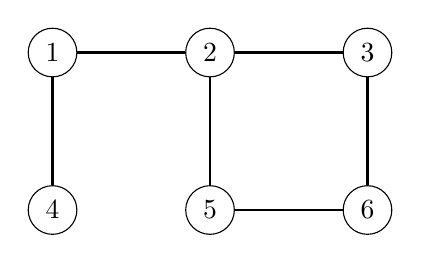
\begin{tikzpicture}
\node[draw, circle] (1) at (1,5) {$1$};
\node[draw, circle] (2) at (3,5) {$2$};
\node[draw, circle] (3) at (5,5) {$3$};
\node[draw, circle] (4) at (1,3) {$4$};
\node[draw, circle] (5) at (3,3) {$5$};
\node[draw, circle] (6) at (5,3) {$6$};

\path[draw,thick,-] (1) -- (2);
\path[draw,thick,-] (2) -- (3);
\path[draw,thick,-] (1) -- (4);
\path[draw,thick,-] (3) -- (6);
\path[draw,thick,-] (2) -- (5);
\path[draw,thick,-] (5) -- (6);
\end{tikzpicture}
\end{center}
Supongamos que la búsqueda comienza en el nodo 1.
Primero, procesamos todos los nodos que se pueden alcanzar
desde el nodo 1 usando una sola arista:
\begin{center}
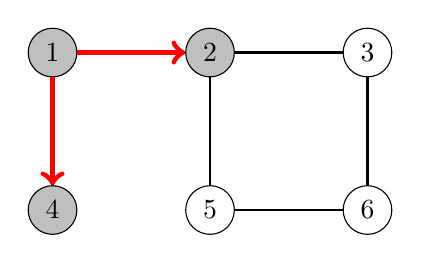
\begin{tikzpicture}
\node[draw, circle,fill=lightgray] (1) at (1,5) {$1$};
\node[draw, circle,fill=lightgray] (2) at (3,5) {$2$};
\node[draw, circle] (3) at (5,5) {$3$};
\node[draw, circle,fill=lightgray] (4) at (1,3) {$4$};
\node[draw, circle] (5) at (3,3) {$5$};
\node[draw, circle] (6) at (5,3) {$6$};

\path[draw,thick,-] (1) -- (2);
\path[draw,thick,-] (2) -- (3);
\path[draw,thick,-] (1) -- (4);
\path[draw,thick,-] (3) -- (6);
\path[draw,thick,-] (2) -- (5);
\path[draw,thick,-] (5) -- (6);

\path[draw,thick,-] (1) -- (2);
\path[draw,thick,-] (2) -- (3);
\path[draw,thick,-] (1) -- (4);
\path[draw,thick,-] (2) -- (5);

\path[draw=red,thick,->,line width=2pt] (1) -- (2);
\path[draw=red,thick,->,line width=2pt] (1) -- (4);
\end{tikzpicture}
\end{center}
Después de esto, procedemos a los nodos 3 y 5:
\begin{center}
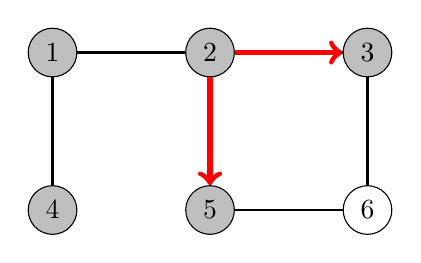
\begin{tikzpicture}
\node[draw, circle,fill=lightgray] (1) at (1,5) {$1$};
\node[draw, circle,fill=lightgray] (2) at (3,5) {$2$};
\node[draw, circle,fill=lightgray] (3) at (5,5) {$3$};
\node[draw, circle,fill=lightgray] (4) at (1,3) {$4$};
\node[draw, circle,fill=lightgray] (5) at (3,3) {$5$};
\node[draw, circle] (6) at (5,3) {$6$};

\path[draw,thick,-] (1) -- (2);
\path[draw,thick,-] (2) -- (3);
\path[draw,thick,-] (1) -- (4);
\path[draw,thick,-] (3) -- (6);
\path[draw,thick,-] (2) -- (5);
\path[draw,thick,-] (5) -- (6);

\path[draw,thick,-] (1) -- (2);
\path[draw,thick,-] (2) -- (3);
\path[draw,thick,-] (1) -- (4);
\path[draw,thick,-] (2) -- (5);

\path[draw=red,thick,->,line width=2pt] (2) -- (3);
\path[draw=red,thick,->,line width=2pt] (2) -- (5);
\end{tikzpicture}
\end{center}
Finalmente, visitamos el nodo 6:
\begin{center}
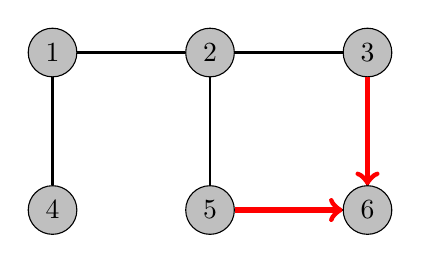
\begin{tikzpicture}
\node[draw, circle,fill=lightgray] (1) at (1,5) {$1$};
\node[draw, circle,fill=lightgray] (2) at (3,5) {$2$};
\node[draw, circle,fill=lightgray] (3) at (5,5) {$3$};
\node[draw, circle,fill=lightgray] (4) at (1,3) {$4$};
\node[draw, circle,fill=lightgray] (5) at (3,3) {$5$};
\node[draw, circle,fill=lightgray] (6) at (5,3) {$6$};

\path[draw,thick,-] (1) -- (2);
\path[draw,thick,-] (2) -- (3);
\path[draw,thick,-] (1) -- (4);
\path[draw,thick,-] (3) -- (6);
\path[draw,thick,-] (2) -- (5);
\path[draw,thick,-] (5) -- (6);

\path[draw,thick,-] (1) -- (2);
\path[draw,thick,-] (2) -- (3);
\path[draw,thick,-] (1) -- (4);
\path[draw,thick,-] (2) -- (5);

\path[draw=red,thick,->,line width=2pt] (3) -- (6);
\path[draw=red,thick,->,line width=2pt] (5) -- (6);
\end{tikzpicture}
\end{center}
Ahora hemos calculado las distancias
desde el nodo inicial a todos los nodos del grafo.
Las distancias son las siguientes:

\begin{tabular}{ll}
\\
nodo & distancia \\
\hline
1 & 0 \\
2 & 1 \\
3 & 2 \\
4 & 1 \\
5 & 2 \\
6 & 3 \\
\\
\end{tabular}

Al igual que en la búsqueda en profundidad,
la complejidad temporal de la búsqueda en anchura
es $O(n+m)$, donde $n$ es el número de nodos
y $m$ es el número de aristas.

\subsubsection*{Implementación}

La búsqueda en anchura es más difícil
de implementar que la búsqueda en profundidad,
porque el algoritmo visita nodos
en diferentes partes del grafo.
Una implementación típica se basa en
una cola que contiene nodos.
En cada paso, el siguiente nodo en la cola
será procesado.

El siguiente código asume que el grafo está almacenado
como listas de adyacencia y mantiene las siguientes
estructuras de datos:
\begin{lstlisting}
queue<int> q;
bool visitado[N];
int distancia[N];
\end{lstlisting}

La cola \texttt{q}
contiene los nodos a procesar
en orden creciente de su distancia.
Los nuevos nodos siempre se agregan al final
de la cola, y el nodo al principio
de la cola es el siguiente nodo a procesar.
El arreglo \texttt{visitado} indica
qué nodos ya ha visitado la búsqueda,
y el arreglo \texttt{distancia} contendrá las
distancias desde el nodo inicial hasta todos los nodos del grafo.

La búsqueda se puede implementar de la siguiente manera,
comenzando desde el nodo $x$:
\begin{lstlisting}
visitado[x] = true;
distancia[x] = 0;
q.push(x);
while (!q.empty()) {
    int s = q.front(); q.pop();
    // procesar nodo s
    for (auto u : adj[s]) {
        if (visitado[u]) continue;
        visitado[u] = true;
        distancia[u] = distancia[s]+1;
        q.push(u);
    }
}
\end{lstlisting}

\section{Aplicaciones}

Usando los algoritmos de recorrido de grafos,
podemos comprobar muchas propiedades de los grafos.
Normalmente, tanto la búsqueda en profundidad como
la búsqueda en amplitud pueden ser utilizadas,
pero en la práctica, la búsqueda en profundidad
es una mejor opción, porque es
más fácil de implementar.
En las siguientes aplicaciones asumiremos que el grafo es no dirigido.

\subsubsection{Comprobación de conectividad}

\index{grafo conectado}

Un grafo es conectado si existe un camino
entre cualquier par de nodos del grafo.
Así que podemos comprobar si un grafo es conectado
comenzando desde un nodo arbitrario y
descubriendo si podemos alcanzar todos los demás nodos.

Por ejemplo, en el grafo
\begin{center}
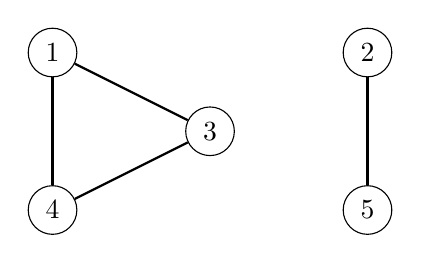
\begin{tikzpicture}
\node[draw, circle] (2) at (7,5) {$2$};
\node[draw, circle] (1) at (3,5) {$1$};
\node[draw, circle] (3) at (5,4) {$3$};
\node[draw, circle] (5) at (7,3) {$5$};
\node[draw, circle] (4) at (3,3) {$4$};

\path[draw,thick,-] (1) -- (3);
\path[draw,thick,-] (1) -- (4);
\path[draw,thick,-] (3) -- (4);
\path[draw,thick,-] (2) -- (5);
\end{tikzpicture}
\end{center}
una búsqueda en profundidad desde el nodo $1$ visita
los siguientes nodos:
\begin{center}
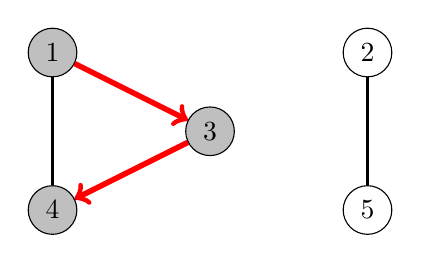
\begin{tikzpicture}
\node[draw, circle] (2) at (7,5) {$2$};
\node[draw, circle,fill=lightgray] (1) at (3,5) {$1$};
\node[draw, circle,fill=lightgray] (3) at (5,4) {$3$};
\node[draw, circle] (5) at (7,3) {$5$};
\node[draw, circle,fill=lightgray] (4) at (3,3) {$4$};

\path[draw,thick,-] (1) -- (3);
\path[draw,thick,-] (1) -- (4);
\path[draw,thick,-] (3) -- (4);
\path[draw,thick,-] (2) -- (5);

\path[draw=red,thick,->,line width=2pt] (1) -- (3);
\path[draw=red,thick,->,line width=2pt] (3) -- (4);

\end{tikzpicture}
\end{center}

Como la búsqueda no visitó todos los nodos,
podemos concluir que el grafo no está conectado.
De manera similar, también podemos encontrar todos los componentes conectados
de un grafo iterando sobre los nodos y siempre
comenzando una nueva búsqueda en profundidad si el nodo actual
no pertenece a ningún componente aún.

\subsubsection{Encontrar ciclos}

\index{ciclo}

Un grafo contiene un ciclo si durante un recorrido del grafo,
encontramos un nodo cuyo vecino (distinto del
nodo anterior en el camino actual) ya ha sido
visitado.
Por ejemplo, el grafo
\begin{center}
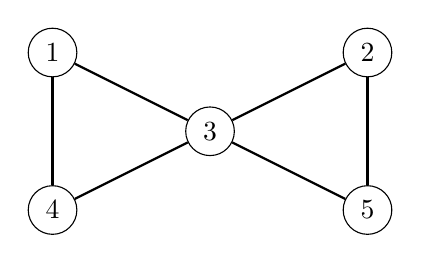
\begin{tikzpicture}
\node[draw, circle] (2) at (7,5) {$2$};
\node[draw, circle] (1) at (3,5) {$1$};
\node[draw, circle] (3) at (5,4) {$3$};
\node[draw, circle] (5) at (7,3) {$5$};
\node[draw, circle] (4) at (3,3) {$4$};

\path[draw,thick,-] (1) -- (3);
\path[draw,thick,-] (1) -- (4);
\path[draw,thick,-] (3) -- (4);
\path[draw,thick,-] (2) -- (5);
\path[draw,thick,-] (2) -- (3);
\path[draw,thick,-] (3) -- (5);
\end{tikzpicture}
\end{center}
contiene dos ciclos y podemos encontrar uno
de ellos de la siguiente manera:
\begin{center}
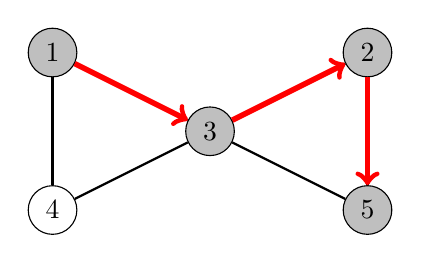
\begin{tikzpicture}
\node[draw, circle,fill=lightgray] (2) at (7,5) {$2$};
\node[draw, circle,fill=lightgray] (1) at (3,5) {$1$};
\node[draw, circle,fill=lightgray] (3) at (5,4) {$3$};
\node[draw, circle,fill=lightgray] (5) at (7,3) {$5$};
\node[draw, circle] (4) at (3,3) {$4$};

\path[draw,thick,-] (1) -- (3);
\path[draw,thick,-] (1) -- (4);
\path[draw,thick,-] (3) -- (4);
\path[draw,thick,-] (2) -- (5);
\path[draw,thick,-] (2) -- (3);
\path[draw,thick,-] (3) -- (5);

\path[draw=red,thick,->,line width=2pt] (1) -- (3);
\path[draw=red,thick,->,line width=2pt] (3) -- (2);
\path[draw=red,thick,->,line width=2pt] (2) -- (5);

\end{tikzpicture}
\end{center}
Después de movernos del nodo 2 al nodo 5, notamos que
el vecino 3 del nodo 5 ya ha sido visitado.
Así, el grafo contiene un ciclo que pasa por el nodo 3,
por ejemplo, $3 \rightarrow 2 \rightarrow 5 \rightarrow 3$.

Otra forma de saber si un grafo contiene un ciclo
es simplemente calcular el número de nodos y aristas
en cada componente.
Si una componente contiene $c$ nodos y no tiene ciclo,
debe contener exactamente $c-1$ aristas
(es decir, debe ser un árbol).
Si hay $c$ o más aristas, la componente
seguramente contiene un ciclo.

\subsubsection{Comprobación de propiedad de ser bipartito}

\index{grafo bipartito}

Un grafo es bipartito si sus nodos pueden ser coloreados
usando dos colores de manera que no haya nodos adyacentes
con el mismo color.
Es sorprendentemente fácil comprobar si un grafo
es bipartito utilizando algoritmos de recorrido de grafos.

La idea es colorear el nodo inicial de azul,
todos sus vecinos de rojo, todos sus vecinos de azul, y así sucesivamente.
Si en algún punto del recorrido notamos que
dos nodos adyacentes tienen el mismo color,
esto significa que el grafo no es bipartito.
De lo contrario, el grafo es bipartito y se ha encontrado una coloración
válida.

Por ejemplo, el grafo
\begin{center}
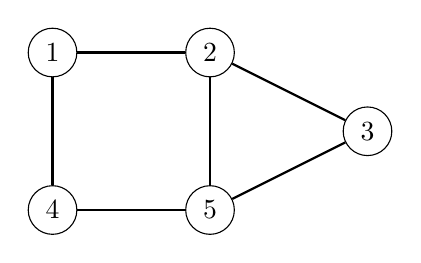
\begin{tikzpicture}
\node[draw, circle] (2) at (5,5) {$2$};
\node[draw, circle] (1) at (3,5) {$1$};
\node[draw, circle] (3) at (7,4) {$3$};
\node[draw, circle] (5) at (5,3) {$5$};
\node[draw, circle] (4) at (3,3) {$4$};

\path[draw,thick,-] (1) -- (2);
\path[draw,thick,-] (2) -- (5);
\path[draw,thick,-] (5) -- (4);
\path[draw,thick,-] (4) -- (1);
\path[draw,thick,-] (2) -- (3);
\path[draw,thick,-] (5) -- (3);
\end{tikzpicture}
\end{center}
no es bipartito, porque una búsqueda desde el nodo 1
procede de la siguiente manera:
\begin{center}
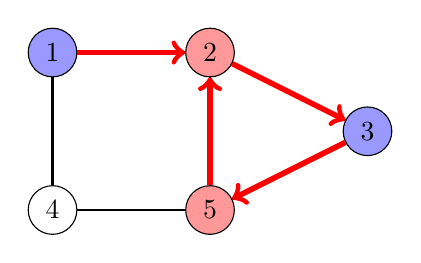
\begin{tikzpicture}
\node[draw, circle,fill=red!40] (2) at (5,5) {$2$};
\node[draw, circle,fill=blue!40] (1) at (3,5) {$1$};
\node[draw, circle,fill=blue!40] (3) at (7,4) {$3$};
\node[draw, circle,fill=red!40] (5) at (5,3) {$5$};
\node[draw, circle] (4) at (3,3) {$4$};

\path[draw,thick,-] (1) -- (2);
\path[draw,thick,-] (2) -- (5);
\path[draw,thick,-] (5) -- (4);
\path[draw,thick,-] (4) -- (1);
\path[draw,thick,-] (2) -- (3);
\path[draw,thick,-] (5) -- (3);

\path[draw=red,thick,->,line width=2pt] (1) -- (2);
\path[draw=red,thick,->,line width=2pt] (2) -- (3);
\path[draw=red,thick,->,line width=2pt] (3) -- (5);
\path[draw=red,thick,->,line width=2pt] (5) -- (2);
\end{tikzpicture}
\end{center}
Notamos que el color de los nodos 2 y 5
es rojo, mientras que son nodos adyacentes en el grafo.
Por lo tanto, el grafo no es bipartito.

Este algoritmo siempre funciona, porque cuando
solo hay dos colores disponibles,
el color del nodo inicial en una componente
determina los colores de todos los demás nodos en la componente.
No importa si el
nodo inicial es rojo o azul.

Nota que en el caso general,
es difícil saber si los nodos
en un grafo pueden ser coloreados usando $k$ colores
de manera que no haya nodos adyacentes con el mismo color.
Incluso cuando $k=3$, no se conoce un algoritmo eficiente
pero el problema es NP-hard.
